\documentclass{article}
\usepackage{graphicx}
\usepackage{hyperref}
\usepackage[a4paper, total={7in, 10in}]{geometry} %6,10
\usepackage{float}
\usepackage[utf8]{inputenc}
\usepackage{listings}
\usepackage{xcolor}
\usepackage{amsmath}
\usepackage{amssymb}
\usepackage{multicol}
\usepackage{enumerate}
\usepackage{tikz}
\usepackage{mathtools}
\newcommand*{\horzbar}{\rule[.5ex]{2.5ex}{0.5pt}}    % horizontal bar in matrices

\newcommand\undermat[2]{%
  \makebox[0pt][l]{$\smash{\underbrace{\phantom{%
    \begin{matrix}#2\end{matrix}}}_{\text{$#1$}}}$}#2}

\title{Numerical analysis for machine learning}
\author{Lorenzo Bozzoni}
\date{\today}

\begin{document}
\maketitle
\tableofcontents
\section{Basic concepts of linear algebra}
The following are the main concepts of linear algebra we are going to face during the starting phase of the course:
\begin{enumerate}
    \item Linear systems of equations: $A\underline{x} = \underline{b}$
    \item Eigenvalues and eigenvectors: $A\underline{x} = \lambda \underline{x}$
    \item Singular value decomposition (SVD):$A\underline{v} = \sigma u$
    \item Minimization problem
    \item Factorization: $PA = LU$
\end{enumerate}


% $\mathbb{A}\underline{x} = \lambda \underline{x}$
% $\mathbb{A}\underline{v} = \sigma \mathbb{u}$

\section{Matrix-vector multiplication}
\[
\underline{c} = \underbrace{\begin{bmatrix}
    1 & 2\\
    3 & 4\\
    5 & 6
\end{bmatrix}}_{A_1}
\underbrace{\begin{bmatrix}
    x_1\\
    x_2
\end{bmatrix}}_{\underline{x}}
= 
\begin{bmatrix}
    1x_1 + 2x_2\\
    3x_1 + 4x_2\\
    5x_1 + 6x_2 
\end{bmatrix}
=
\underbrace{
\begin{bmatrix}
    1\\
    2\\
    3
\end{bmatrix}
x_1+
\begin{bmatrix}
    4\\
    5\\
    6
\end{bmatrix}
x_2
}_{\text{linear combination}}
\]
We say that the vector $\underline{c}$ belongs to the \textbf{column space} of $A_1$, i.e. $\underline{c} \in \mathcal{C}(A_1)$.
\[
\overbrace{
\underbrace{
\begin{bmatrix}
    1 & 4 & 7\\
    2 & 5 & 8\\
    3 & 6 & 9
\end{bmatrix}}_{\underline{a_1} \hspace{0.2cm} \underline{a_2} \hspace{0.2cm} \underline{a_3}}
}^{A_2}
\begin{bmatrix}
    x_1\\
    x_2\\
    x_3
\end{bmatrix}
\]
In this case we can easily notice that $\underline{a_3} = \underline{a_1} + \underline{a_2}$, which means that one column can be expressed as a linear combination of the other two (this means that the matrix $A_2$ is singular). Because of this, we can say that $\mathcal{C}(A_2) = \mathcal{C}(A_1)$, i.e. the column space of $A_2$ is the same as the column space of $A_1$.

Those columns spaces are a plane passing through the origin and spanned by the two vectors $\underline{a_1}$ and $\underline{a_2}$ (they define the slope of that plane).

Let's now consider these matrix:
\[
\underbrace{
\begin{bmatrix}
    1 & 4 & 7\\
    2 & 5 & 8\\
    3 & 6 & 10
\end{bmatrix}
}_{A_3} 
\hspace{3cm}
\underbrace{
\begin{bmatrix}
    1 & 2 & 3\\
    2 & 4 & 6\\
    3 & 6 & 9
\end{bmatrix}
}_{A_4} 
\]
This left-hand matrix column space is $\mathcal{C}(A_3) = \mathbb{R}^3$, i.e. the entire real space of three dimensions. This is because the three vector columns of $A_3$ are linearly independet so they span the entire space and not just a plane.
While the column space of $A_4$ is instead: $\mathcal{C}(A_3) = \begin{bmatrix}
    1&2&3
\end{bmatrix}^T$ i.e. just a line since the three columns are linearly dependent and so they lie on the same line (they are parallel) just with different magnitude.

Another measure regarding matrices is the \textbf{dimension} or \textbf{rank}:
\begin{itemize}
    \item $rank(A_1) = 2$
    \item $rank(A_2) = 2$
    \item $rank(A_3) = 3$
    \item $rank(A_4) = 1$
\end{itemize}
The rank is the number of linearly independent columns (or rows) of a matrix.

Let's consider again the matrix $A_3$:
\[
\begin{bmatrix}
    1 & 4 & 7\\
    2 & 5 & 8\\
    3 & 6 & 10
\end{bmatrix}
\begin{bmatrix}
    x_1\\
    x_2\\
    x_3
\end{bmatrix}
= 
\underbrace{\begin{bmatrix}
    1\\
    2\\
    3
\end{bmatrix}
x_1+
\begin{bmatrix}
    4\\
    5\\
    6
\end{bmatrix}
x_2+
\begin{bmatrix}
    7\\
    8\\
    10
\end{bmatrix}
x_3}_{\in \mathcal{C}(A_3)}
=
\begin{bmatrix}
    b_1\\
    b_2\\
    b_3
\end{bmatrix}
\]
so $\underline{b}$ must be in $\mathcal{C}(A_3)$ in order to have the system solvable. If $\underline{b} \notin \mathcal{C}(A_3)$, then the system is not solvable. In this particular case we have that the columns of $A_3$ are linearly independent, so the system is solvable for any $\underline{b}$ because $\mathcal{C}(A_3) = \mathbb{R}^3$ and so $\underline{b}$ is for sure inside that space. \\

Given A, find $\mathcal{C}(A)$. How can we solve this problem? Considering $\underline{a_1}, \dots, \underline{a_n}$ as A columns, we can use the following iterative algorithm:
\begin{itemize}
    \item put $\underline{a_1}$ in $\mathcal{C}(A)$
    \item if $\underline{a_2} = \alpha \underline{a_1} \rightarrow \underline{a_2} \notin \mathcal{C}(A)$, otherwise put $\underline{a_2}$ in $\mathcal{C}(A)$
\end{itemize}
Until you reach the last column.

\subsection{Row-reduced echelon form}
Given the matrix $A$, defined as follow:
\[
A = \begin{bmatrix}
    1 & 4 & 7\\
    2 & 5 & 8\\
    3 & 6 & 9
\end{bmatrix}
\]
we can obtain the \textbf{row-reduced echelon form} of $A$ by applying the following operations:
\[
A = CR = \begin{bmatrix}
1 & 4\\
2 & 5\\
3 & 6
\end{bmatrix}
\begin{bmatrix}
    1 & 0 & -1\\
    0 & 1 & 2
\end{bmatrix}
\]
where $C$ is the matrix containing the columns of $A$ that are linearly independent (i.e. $\mathcal{C}(A)$) and $R$ is the matrix of the coefficients of the linear combination of the columns of $A$ that gives the columns of $C$.\\

Let's now consider the following matrix:
\[
A_1 = \begin{bmatrix}
1 & 4\\
2 & 5\\
3 & 6
\end{bmatrix}  
\hspace{2cm}
A_1^\intercal = \begin{bmatrix}
1 & 2 & 3\\
4 & 5 & 6
\end{bmatrix}  
\]
What we can say about $A_1^\intercal$ column space? Is there any relationship with the column space of $A_1$?

In order to compute its column space, we can start noticing that: $\underline{a_3} = 2\underline{a_2} - \underline{a_1}$. So, in general, we can say that:
\[
dim(\mathcal{C}(A)) = dim(\mathcal{C}(A^\intercal)) = r \leq n \hspace{1cm} \text{where $n$ is the number of columns of $A$}
\]

\section{Matrix-matrix multiplication}
\[
C = AB = \begin{bmatrix}
    \vline & \vline & \vline\\
    \underline{a_1} & \ldots & \underline{a_n}\\
    \vline & \vline & \vline
\end{bmatrix}
\begin{bmatrix}
    \horzbar & \underline{b_1} & \horzbar\\
    \horzbar & \vdots & \horzbar\\
    \horzbar & \underline{b_n} & \horzbar
\end{bmatrix}
= \overset{\overset{\text{col}}{\downarrow}}{\underline{a_1}}\overset{\overset{\text{row}}{\downarrow}}{\underline{b_1}} + \dots + \underline{a_n}\underline{b_n}
\] 
All the products that are summed at the end of the equation are matrices of rank 1. 

Example:
\[
\begin{bmatrix}
1 & 2\\
3 & 4
\end{bmatrix}  
\begin{bmatrix}
    2 & 1\\
    2 & 3
\end{bmatrix}
= \underbrace{
    \begin{bmatrix}
        2 & 1\\
        6 & 3
    \end{bmatrix}
}_{\text{rank = 1}}
+ \underbrace{
    \begin{bmatrix}
        4 & 6\\
        8 & 12
    \end{bmatrix}
}_{\text{rank = 1}}
= \begin{bmatrix}
    6 & 7\\
    14 & 15
\end{bmatrix}
\]


\section{Factorizations}
\begin{enumerate}
    \item $A = LU$ or $PA = LU$
    \item $A = QR$ where $Q$ is orthogonal and $R$ is upper triangular
    This is an improved version of the Row-reduced echelon form because that worked only for square matrices, while this works for any matrix.
    \item Eigenvalues and eigenvectors decomposition: when $S = S^\intercal$ (symmetric matrix) we can factorize it as $S = Q\Lambda Q^\intercal$ where $\Lambda$ is a diagonal matrix and $Q$ is an orthogonal matrix (they are all squared matrices)
    \item Generalization of the above: $A = X\Lambda X^{-1}$ where $X$ is a non-orthogonal matrix
    \item $A = U\Sigma V^\intercal$ where $U$ and $V$ are orthogonal matrices and $\Sigma$ is a pseudo-diagonal matrix
\end{enumerate}
A matrix is said to be pseudo-diagonal if it has the following form:
\[
    \Sigma = 
    \begin{bmatrix}
        \sigma_1 & 0 & 0 & 0\\
        0 & \sigma_2 & 0 & 0\\
        0 & 0 & \ddots & 0\\
        0 & 0 & 0 & \sigma_n\\
        0 & 0 & 0 & 0\\
        \vdots & \vdots & \vdots & \vdots\\
        0 & 0 & 0 & 0
    \end{bmatrix}
    \hspace{2cm}
    m \text{ rows} \times n \text{ columns}
\]
So it has diagonal elements for the first $n$ rows then it has all zeros.

\subsection{Orthogonal matrices}
A matrix $Q$ is orthogonal if $Q^\intercal Q = I$ (i.e. $Q^\intercal = Q^{-1}$). This means that the columns of $Q$ are orthonormal, i.e. they are orthogonal and have unit norm.\\

The determinant of a orthogonal matrix is $\pm 1$.

Properties:
\begin{itemize}
    \item $||Q\underline{x}|| = ||\underline{x}||$
    \item $||Q\underline{x}||^2 = (Q\underline{x})^\intercal Q\underline{x} = \underline{x}^\intercal \underbrace{Q^\intercal Q}_{I} \underline{x} = ||\underline{x}||^2$
\end{itemize}
The first property is particularly easy to interpret since it means that when we multiply an orthogonal matrix to a vector, the norm of the vector doesn't change. As a proof of this, we can consider the following examples:

\subsubsection{Rotation}
A classical rotation matrix is:
\[
\begin{bmatrix}
    cos(\theta) & -sin(\theta)\\
    sin(\theta) & cos(\theta)
\end{bmatrix}    
\]
\subsubsection{Reflection}
\begin{center}
    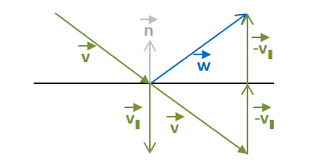
\includegraphics[scale=0.5]{images/Reflection.png}
\end{center}
The horizontal line in the figure represent a plane $\pi$ while $\underline{n}$ is its normal vector of length 1. 
Given $\underline{v}$ to obtain $\underline{w}$ we can use the following formula:
\[
\underline{w} = \underline{v} - 2(\underline{v}^\intercal \underline{n})\underline{n} = \underbrace{(I - 2\underline{n}\underline{n}^\intercal)}_{\text{reflection matrix}}\underline{v}
\]
Moreover, the reflection matrix $R$ is not only orthogonal, but also the inverse of itself, i.e. $R^{-1} = R^\intercal$. This makes sense because if we apply the reflection matrix twice, we obtain the original vector $\underline{v}$, i.e. the reflection of the reflection is the starting vector.

If we didn't have the 2 in the formula, we would obtain the projection of $\underline{v}$ on the plane $\pi$ which is called orthogonal projection and the matrix $R$ would be singular. \\

Let's now dive a bit into the third point of the factorization list. We said that when $S = S^\intercal$ (symmetric matrix) we can factorize it as $S = Q\Lambda Q^\intercal$ where $\Lambda$ is a diagonal matrix and $Q$ is an orthogonal matrix.\\
\[
S = S^\intercal = \underbrace{(Q\Lambda))}_{\tilde{Q}}Q^\intercal = \tilde{Q}Q^\intercal   
\]
\[
\tilde{Q} = \underline{q_1}\underline{\lambda_1} + \dots + \underline{q_n}\underline{\lambda_n}    
\]
Where the $q$ vectors are columns and $\lambda$ vectors are rows.
So we can reformulate:
\[
    S = (\underline{q_1}\underline{\lambda_1} + \dots + \underline{q_n}\underline{\lambda_n})Q^\intercal = \underline{q_1}\underline{\lambda_1}\underline{q_1}^\intercal + \dots + \underline{q_n}\underline{\lambda_n}\underline{q_n}^\intercal
\]
This is called \textbf{spectral decomposition} of matrix $S$ and $q_1, \dots, q_n$ are the eigenvectors of $S$ while $\lambda_1, \dots, \lambda_n$ are the eigenvalues of $S$.
\[
    S\underline{q_1} = \lambda_1\underline{q_1} = (\underline{q_1}\underline{\lambda_1}\underline{q_1}^\intercal + \dots + \underline{q_n}\underline{\lambda_n}\underline{q_n}^\intercal)\underline{q_1} = 
    \underline{\lambda_1}\underline{q_1}(\underline{q_1^\intercal}\underline{q_1})
    \]
All the other products are null since the vector $\underline{q_1}$ is orthogonal to all the other vectors $\underline{q_i}$ for $i \neq 1$ (recall that they are eigenvectors).

\section{Null spaces}
Let's consider the starting problem for a linear system of equations:
\[
A\underline{x} = \underline{b} \hspace{1cm} \text{with} \hspace{1cm} A\in \mathbb{R}^{m \times n}, \text{rank($A$)}=r    
\]

We are going to introduce 2 more spaces other than the column ones. To do so we consider:
\[
  A\underline{x} = \underline{0} \hspace{1cm} \rightarrow \hspace{1cm} N(A) \equiv \ker(A) = \{\underline{x} \in \mathbb{R}^n : A\underline{x} = \underline{0}\}  
\]
\[
    A^\intercal\underline{x} = \underline{0} \hspace{1cm} \rightarrow \hspace{1cm} N(A^\intercal) \equiv \ker(A^\intercal) = \{\underline{x} \in \mathbb{R}^n : A^\intercal\underline{x} = \underline{0}\}    
\]

So now, adding the so called \textbf{null spaces} we have that:
\begin{enumerate}
    \item $\mathcal{C}(A) \subset  \mathbb{R}^m$ and $dim(\mathcal{C}(A)) = r$
    \item $\mathcal{C}(A^\intercal) \subset \mathbb{R}^n$ and $dim(\mathcal{C}(A^\intercal)) = r$
    \item $N(A) \subset \mathbb{R}^n$ and $dim(N(A)) = ?$
    \item $N(A^\intercal) \subset \mathbb{R}^m$ and $dim(N(A^\intercal)) = ?$
\end{enumerate}
We still do not know the dimensions of those spaces. \\

\textbf{Example}\\
\[
A = \begin{bmatrix}
    1 & 4 & 7\\
    2 & 5 & 8\\
    3 & 6 & 9
\end{bmatrix}
\begin{bmatrix}
    x_1\\
    x_2\\
    x_3
\end{bmatrix}
= 
\begin{bmatrix}
    0\\
    0\\
    0
\end{bmatrix}
\hspace{0.3cm} \implies \hspace{0.3cm}
\begin{cases}
    x_1 + 4x_2 + 7x_3 = 0\\
    2x_1 + 5x_2 + 8x_3 = 0\\
    3x_1 + 6x_2 + 9x_3 = 0
\end{cases}    
\]
We compute the first equation
\[
    x_1 = -4x_2 - 7x_3 \hspace{0.3cm} \implies \hspace{0.3cm} \begin{cases}
        -3x_2 - 6x_3 = 0\\
        -6x_2 - 12x_3 = 0
    \end{cases}
\]
What is important to notice is that $A$ has rank$=2$ so we have $3-2=1$  \textbf{degrees of freedom}, i.e. we can choose one variable and the other two are automatically defined. This is visible in the last two equations of the system for example. 
In general, the degrees of freedom are given by $n-r$ where $n$ is the number of columns of $A$ and $r$ is the rank of $A$.\\

If we had 10 instead of 9 in $A$ we would have had $3-3=0$ degrees of freedom. This would translate in having the matrix $A$ full rank and $N(A) = \{\underline{0}\}$ so the only solution would be the null vector.


\section{Null space cardinality}
In the first lecture, we defined 4 spaces: $N(A), N(A^\intercal), \mathcal{C}(A), \mathcal{C}(A^\intercal)$. For the last two we defined also their cardinality whilst for the first ones we weren't able to tell yet. In this lecture we are going to find those values and prove them. In order to do so, we start from few useful properties:
\begin{enumerate}
    \item $\underline{x} = \underline{0} \in N(A)$ for any matrix $A$
    \item if $\underline{x}, \underline{y} \in N(A) \implies A(\underline{x} + \underline{y}) = \underline{0}$
    \item if $\underline{x} \in N(A) \implies \alpha\underline{x}$ with $\alpha \in \mathbb{R} \implies A(\alpha\underline{x}) = \underline{0}$
\end{enumerate}  

Consider, once again, the matrix $A \in \mathbb{R}^{m\times n}$, rank($A$) = $r \leq n$. 
We have seen the decomposition $A = CR$, where $C$ contains the linearly independent columns of $A$ and $R$ contains the coefficients that allow to recover the columns of $A$ starting from its independent columns. 
So, the matrix $A$ can be rewritten as:
\[
  A = \begin{bmatrix}
    A_1 & A_2
  \end{bmatrix} 
  \hspace{1cm}
  A_1 \in \mathbb{R}^{m\times r} \hspace{1cm} A_2 \in \mathbb{R}^{m\times (n-r)} 
\]
Where $A_1$ contains the independent columns of $A$ and $A_2$ the dependent ones.
Example:
\[
A = 
\begin{bmatrix}
    1 & 4 & 7\\
    2 & 5 & 8\\
    3 & 6 & 9
\end{bmatrix}
= 
\underbrace{
\begin{bmatrix}
1 & 4\\
2 & 5\\
3 & 6
\end{bmatrix}}_{A_1}
\begin{bmatrix}
    1 & 0 & -1\\
    0 & 1 & \undermat{B}{2}
\end{bmatrix}
\]
Since we have the last column of $A$, that is linearly dependent so it belongs to $A_2$, we can reformulate it in this way:
\[
    A = \begin{bmatrix}
        A_1 & A_2
      \end{bmatrix} 
    = \begin{bmatrix}
        A_1 & A_1B
    \end{bmatrix}
\]
We build a new matrix $K$ defined as follows:
\[
    K = \begin{bmatrix}
        -B\\
        I_{n-r}
    \end{bmatrix}
    \hspace{1cm}
    K \in \mathbb{R}^{n\times(n-r)}    
    \hspace{1cm}
    B \in \mathbb{R}^{r\times(n-r)}    
\]

\[
AK = \begin{bmatrix}
    A_1 & A_1B
\end{bmatrix} 
\begin{bmatrix}
    -B\\
    I_{n-r}
\end{bmatrix}
= A_1(-B) + A_1B = 0   
\]
Where the last 0 is actually a matrix of zeros of dimension $m\times(n-r)$
because A has size $m\times n$ and $K$ has size $n\times(n-r)$.
We have that:
\[
    AK = 0 \implies A\underline{k_i} = 0 \hspace{1cm} \forall i \in \{1, \dots, n-r\}    
\]
Where $k_i$ is the i-th column of $K$. This means that: $\underline{k_i} \in N(A) \hspace{0.2cm} \forall i$.

Now, we want to demonstrate that: $K\underline{u} = 0 \implies \underline{u} = \underline{0}$. 
To do so, we start from expanding $K$ from its definition:
\[
    K = \begin{bmatrix}
        -B\\
        I
    \end{bmatrix}
    \underline{u} = 0
    \implies
    \begin{bmatrix}
        -B\underline{u}\\
        \underline{u}
    \end{bmatrix}
    = 
    \begin{bmatrix}
        \underline{0}\\
        \underline{0}
    \end{bmatrix}
\]
Where the two zero vectors have dimension $r$ and $n-r$ respectively! Considering the second row of the matrix we get: $\underline{u} = \underline{0}$ so all columns of $K$ are linearly independent.\\

If we consider the problem ($\star$) $A\underline{x} = \underline{0}$, we want to prove that each \underline{x} that satisfy ($\star$) must be a linear combination of the columns of $K$.\\
\[
    A_1\underline{x} = \underline{0} \in \mathbb{R}^m \implies \underline{x} = \underline{0} \in \mathbb{R}^r    
\]
Because $A_1$ has linearly independent columns, i.e. has full rank.
\[
    A\underline{u} = \underline{0} \in \mathbb{R}^m \implies \begin{bmatrix}
        A_1 & A_1B
    \end{bmatrix} 
    \begin{bmatrix}
        \underline{u_1}\\
        \underline{u_2}
    \end{bmatrix}  
    = 
    \begin{bmatrix}
        A_1\underline{u_1} + A_1B\underline{u_2}\\
    \end{bmatrix}
    = 
    A_1\left[\underline{u_1} + B\underline{u_2}\right]
    = \underline{0}
\]
We can notice that the last formulation obtained in the equation has the same form as the one from where we started the prove, so we can say that:
\[
    \underline{u_1} + B\underline{u_2} = \underline{0} \implies \underline{u_1} = -B\underline{u_2}    
\]
\[
   \underline{u} = \begin{bmatrix}
    -B\underline{u_2}\\
    \underline{u_2}
\end{bmatrix}
    =
\underbrace{\begin{bmatrix}
    -B\\
    I
\end{bmatrix}}_{K}
    \underline{u_2}
    = K\underline{u_2}
    \implies 
    dim(N(A)) = n - r
\]


\begin{center}
    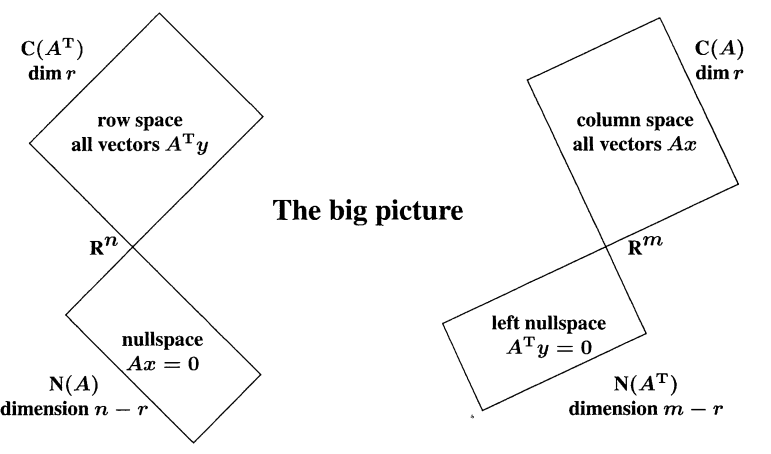
\includegraphics[scale = 0.4]{../images/SpacesDimensions.png}
\end{center}


\section{Eigenvalues and eigenvectors}
Start considering a generic square matrix $n \times n$. We are going later to discuss even the simmetry and positive definite properties.
Here below are the vectorial and the matrix form of the eigenvalue problem:
\[
    A\underline{x_i} = \lambda_i\underline{x_i} \hspace{0.5cm} i = 1, \dots, n \hspace{1cm} X^{-1}AX = \Lambda
\]
Where in the right-hand side there is a diagonal matrix $\Lambda$ with the eigenvalues of $A$ on the diagonal while the matrix $X$ with the eigenvectors of $A$ as columns.\\

\subsection{Eigenvectors of matrix power}
What can we say about the eigenvectors and eigenvalues of $A^2$?
\[
    A^2\underline{x_i} = A(A\underline{x_i}) = A(\lambda_i\underline{x_i}) = \lambda_i(A\underline{x_i}) = \lambda_i^2\underline{x_i}    
\]
So the eigenvalues of $A^2$ are the eigenvalues of $A$ squared.This is valid for any power of $A$ since this method can be applied recursively and it is very useful when there are problems in which a matrix is iteratively multiplied many times. \\

\textbf{Important}:\\
Given $A\in \mathbb{R}^{n\times n}$ full rank, then any vector $\underline{v} \in \mathbb{R}^n$ can be written as a linear combination of the eigenvectors ($x_i$) of $A$.\\

\subsection{Power method}
In mathematics, power iteration (also known as the power method) is an eigenvalue algorithm: given a diagonalizable matrix A, the algorithm will produce a number $\lambda$ , which is the greatest (in absolute value) eigenvalue of A, and a nonzero vector v, which is a corresponding eigenvector of $\lambda$ , that is, $Av=\lambda v$. The algorithm is also known as the Von Mises iteration.

There is also an \textbf{inverse PM} which is applied to $A^{-1}$ to find the minimum eigenvalue or also \textbf{PM with a shift} applied to $(A-\alpha I)^{-1}, \alpha \in \mathbb{R}$ to find the closest eigenvalue to $\alpha$. 

Can even be used in "deflation method" iteratively:
\[
    \begin{bmatrix}
        \lambda_1 & \underline{b_1^\intercal}\\
        0 & A_1
    \end{bmatrix}    
\]
the original matrix could be reduced in that form and at every iteration the procedure is applied to the $A_1$ matrix. This works only if we have different eigenvectors (or values) [check].

\subsection{Similar matrices}
Given two matrices $A, B \in \mathbb{R}^n$, they are said to be similar if $B = M^{-1}AM$, with $M$ invertible. 
\[
    \underbrace{M^{-1}AM}_{B}\underline{y} = \lambda \underline{y} \implies A\underbrace{M\underline{y}}_{\underline{w}} = \lambda \underbrace{M\underline{y}}_{\underline{w}} = A\underline{w} = \lambda \underline{w}    
\]
Where $\lambda, \underline{y}$ contain respectively the eigenvalues and the eigenvectors of $B$. What we get from this equation is that \textbf{similar matrices share the same eigenvectors with scaled eigenvalues}.

\subsection{QR factorization}
Here is introduced in the context of eigenvalues. Let's consider a matrix $A \in \mathbb{R}^{m\times n}$ where $m \geq n$ and $rank(A) = n$ (it has all independent columns). We can factorize $A$ in this way:
\[
    A = QR \hspace{1cm} Q \in \mathbb{R}^{m\times n} \hspace{1cm} R \in \mathbb{R}^{n\times n}
\]
Where is $Q$ is an orthogonal matrix and $R$ is an upper triangular matrix.Since we are dealing with eigenvalues and eigenvectors, we are now going to consider the matrix $A$ squared with the dimension $n\times n$.

\subsubsection{QR iteration} 
\[
    A = A^{(0)} = Q^{(0)}R^{(0)}     
\]
\[
    A^{(1)} = {Q^{(0)}}^{\intercal} A^{(0)} Q^{(0)} = Q^{(1)} R^{(1)}    
\]
So, iterating this procedure we get:
\[
    A^{(2)}, \dots, A^{(S)} = \text{is upper triangular}
\]
After S iterations you obtain an upper triangular matrix. The matrices $A, A^{(0)}, A^{(1)}, \dots, A^{(S)}$ are similar, so they share the same eigenvalues.

But, how can i compute $Q$?\\
With the \textbf{Gram-Schmidt} procedure. It works also for non-square matrices.\\
Let's start from a generic matrix $A$:
\[
    A = \begin{bmatrix}
        \vline & \vline & \vline\\
        \underline{a_1} & \ldots & \underline{a_n}\\
        \vline & \vline & \vline
    \end{bmatrix} 
\]
The algorithm is iterative and it is applied to the columns of $A$ in such way:
\[
  \underline{q_1} = \frac{\underline{a_1}}{||\underline{a_1}||}  
\]
The vector $\underline{q_1}$ is obtained by normalizing the first column of $A$, in such manner the new obtained vector will have norm 1.
\[
    \underline{q_2} = \underline{a_2} - \underline{q_1}(\underline{q_1}^\intercal \underline{a_2}) \implies \underline{q_2} = \dfrac{\underline{q_2}}{||\underline{q_2}||}
\]
The second vector is obtained by subtracting from the second column of $A$ the projection of $\underline{a_2}$ on $\underline{q_1}$, in such manner the new vector will be orthogonal to $\underline{q_1}$ and will have norm 1.
\[
    \underline{q_3} = \underline{a_3} - \underline{q_1}(\underline{q_1}^\intercal \underline{a_3}) - \underline{q_2}(\underline{q_2}^\intercal \underline{a_3}) \implies \underline{q_3} = \dfrac{\underline{q_3}}{||\underline{q_3}||}
\]
And so on... Recall that the orthogonality is needed since we want to obtain an orthogonal matrix $Q$ useful for the factorization. With Gram-Schmidt the resulting matrix not only will be orthogonal but also orthonormal, this means that its columns will have norm unitary.\\  
Let's now continue with the factorization journey. We have said in the introduction of types of factorizations that, given $A \in \mathbb{R}^{n\times n}$, we have:
\[
    A = X \Lambda X^{-1}
\]
Where $X$ has as columns the eigenvectors of A, while $\Lambda$ is a diagonal matrix with the eigenvalues of $A$ on the diagonal. Now, let's consider the case where the matrix $S$ is symmetric.
\[
    S \in \mathbb{R}^{n\times n} \hspace{1cm} S = S^\intercal
\]
We can factorize $S$ as follows:
\[
    S = Q \Lambda Q^\intercal
\]
Where $Q$ is orthogonal (this is true only because $S$ is symmtric) and $\Lambda$ is diagonal.
We can prove that $Q$ is orthogonal by:
\begin{enumerate}
    \item Consider the two vectors $\underline{x}, \underline{y}$ such as: $S\underline{x} = \lambda\underline{x}$ and $S\underline{y} = 0\underline{y}$. So, we are saying that both vectors are eigenvectors.
    \[
        \begin{rcases}
            \underline{y} \in N(S)\\
            \underline{x} \in \mathcal{C}(S) = \mathcal{C}(S^{\intercal})    
        \end{rcases}
        \implies \underline{x} \perp \underline{y}
    \]
    This is confirmed also by the scheme done during lecture with the 4 blocks. Notice that we have not specified or made any assumption on the value of $\lambda$.
    \item Similar to point 1, we consider the two vectors $\underline{x}, \underline{y}$ such as: $S\underline{x} = \lambda\underline{x}$ and $S\underline{y} = \alpha\underline{y}$. Now, consider the matrix $(S - \alpha I)$, we can write:
    \[
        (S - \alpha I)\underline{y} = 0\underline{y} \implies \underline{y} \in N(S - \alpha I)
    \]
    \[
        (S - \alpha I)\underline{x} = (\lambda - \alpha)\underline{x} \implies \underline{x} \in \mathcal{C}(S - \alpha I) = \mathcal{C}((S - \alpha I)^{\intercal})
    \]
    So, again we obtain: $\underline{x} \perp \underline{y}$.
\end{enumerate}
There is another property: $\lambda_i \in \mathbb{R}$, so the eigenvalues on the diagonal of $\Lambda$ are real. Proof:
\[
    S\underline{x} = \lambda\underline{x} \implies \overline{\underline{x}}^\intercal S\underline{x} = \lambda\overline{\underline{x}}^\intercal\underline{x}     
\]
The $\overline{\underline{x}}$ represent the conjugate of the vector $\underline{x}$. If that vector has complex components, those elements are conjugated, otherwise, i.e. they are all real, they remain inalterated. In particular, once a complex number is conjugated, the result is a real number, as shown here:
\[
    (a + ib)(a - ib) = (a^2 + b^2) \in \mathbb{R}    
\]
From the previos equation, we obtain:
\[
    \lambda = \frac{\overline{\underline{x}}^\intercal S\underline{x}}{\overline{\underline{x}}^\intercal\underline{x}} \in \mathbb{R}
\]

\subsection{Positive-definite symmetric matrices (SPD)}
Characterizations:
\begin{enumerate}[i]
    \item $\lambda_i > 0 \hspace{0.5cm} \forall i = 1, \dots, n$
    \item $\underline{v}^\intercal S \underline{v} \geq 0 \hspace{0.5cm} \forall \underline{v} \in \mathbb{R}^n$, with equality if and only if $\underline{v} = 0$
    \item Leading determinants are positive. \\
    \begin{multicols}{2}
        \begin{center}
            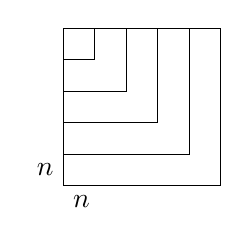
\begin{tikzpicture}
                \draw (0,0) -- (2,0) -- (2,2) -- (0,2) -- (0,0);
                \draw (0,0.4) -- (1.6,0.4) -- (1.6,2) -- (0,2) -- (0,0);
                \draw (0,0.8) -- (1.2,0.8) -- (1.2,2) -- (0,2) -- (0,0); 
                \draw (0,1.2) -- (0.8,1.2) -- (0.8,2) -- (0,2) -- (0,0) node[above left]{$n$};
                \draw (0,1.6) -- (0.4,1.6) -- (0.4,2) -- (0,2) -- (0,0) node[below right]{$n$};
            \end{tikzpicture}
        \end{center}

        This means that the determinant of the matrix obtained by taking the first $k$ rows and columns of $S$ is positive, $\forall k = 1, \dots, n$.
    \end{multicols}

    \item Cholesky decomposition: $S = B^\intercal B$, with $B$ upper triangular
    \item All pivot elements are positive in the Gaussian elimination process
\end{enumerate}

Let's consider $\lambda > 0$ being a certain eigenvalue. 
\[ 
    S\underline{x} = \lambda\underline{x}    
\]
We multiply both sides by $\underline{x}^\intercal$:
\[
    \underline{x}^\intercal S\underline{x} = \lambda\underline{x}^\intercal\underline{x} = \lambda\||\underline{x}\||^2 \geq 0
\]
Recall that $\underline{x}$ is an eigenvector while the before considered vector $\underline{v}$ is a generic vector. With $\underline{v}$, instead, we have:
\[
    \underline{v} = (c_1\underline{x}_1 + c_2\underline{x}_2 + \dots + c_n\underline{x}_n)    
\]
So we are expressing $\underline{v}$ as a linear combination of the eigenvectors of $S$. 
\[
    (c_1\underline{x}_1 + c_2\underline{x}_2 + \dots + c_n\underline{x}_n)^\intercal S (c_1\underline{x}_1 + c_2\underline{x}_2 + \dots + c_n\underline{x}_n)        
\]
\[
    \begin{rcases}
        c_1^2\underline{x}_1^\intercal S \underline{x}_1 = c_1^2\lambda_1\underline{x}_1^\intercal \underline{x}_1 = c_1^2\lambda_1||\underline{x}_1||^2\\
        c_1c_2\underline{x}_1^\intercal S \underline{x}_2 = c_1c_2\lambda_2\underline{x}_1^\intercal \underline{x}_2 = 0\\
    \end{rcases}    
    \text{there are two types of components}
\]
The first components is given by the eigenvectors with the same direction, while the second no so their scalar product is null (they are orthogonal).\\

From \textit{iv}):
\[
    S = B^\intercal B \implies \underline{v}^\intercal(B^\intercal B)\underline{v} = (\underline{v}^\intercal B^\intercal)(B \underline{v}) = (B\underline{v})^\intercal (B\underline{v}) = ||B\underline{v}||^2 \geq 0   
\]

\section{Singular Value Decomposition (SVD)}
We are going to use it for:
\begin{itemize}
    \item Least-squares approximation by introducing the pseudo-inverse of a matrix (Moore-Penrose inverse)
    \item Low-rank approximation with the Eckart-Young theorem
\end{itemize}
We start from:
\[
A \in \mathbb{R}^{m \times n} \hspace{1cm} 
\begin{cases}
m = \text{\# of samples}\\
n = \text{\# of features}
\end{cases}    
\]
We can write:
\[
    A = U\Sigma V^\intercal    
\]
With:
\begin{itemize}
    \item $U$ with dimensions $m \times m$ and orthogonal
    \item $\Sigma$ with dimensions $m \times n$ \textit{almost} diagonal
    \item $V^\intercal$ with dimensions $n \times n$ and orthogonal
\end{itemize}
If $m > n$, we can represent the matrices like this:
\[
\underbrace{
  \begin{bmatrix}
    & & & & & \\
    & & & & & \\
    & & & & & \\
    & & & & & \\
    & & & & & \\
  \end{bmatrix}}_{m \times m}
\underbrace{
  \begin{bmatrix}
    & & & \\
    & & & \\
    & & & \\
    & & & \\
    & & & \\
  \end{bmatrix}}_{m \times n}
\underbrace{
  \begin{bmatrix}
    & & & \\
    & & & \\
    & & & \\
  \end{bmatrix}}_{n \times n}
\]
What is the idea of SVD? Try to change features so variances are maximized and covariances are minimized. We don't want columns to be correlated.\\

In general: rank($A$) = $r < n$.
\[
    AV = U\Sigma \impliedby V^\intercal V = I \impliedby V \text{ is orthogonal}    
\]
The component wise notation is:
\[
    A\underline{v_i} = \sigma_i\underline{u_i}    
\]
Given that the rank of $A$ is $r$:

\[
\begin{bmatrix}
    & & & & & & &\\
    & & & & & & &\\
    & & & & & & &\\
    & & & & & & &\\
    & & & & & & &\\
    & & & & & & &\\
\end{bmatrix}
\begin{bmatrix}
    \sigma_1 & & & &\\
    & \sigma_2 & & &\\
    & & \ddots & &\\
    & & & \sigma_r &\\
    & & & & 0\\
    \hline
    0 & 0 & 0 & 0 & 0\\
    0 & 0 & 0 & 0 & 0\\
\end{bmatrix}
\begin{bmatrix}
    & & & & \\
    & & & & \\
    & & & & \\
    & & & & \\
\end{bmatrix}
\hspace{1cm}
\begin{cases}
\sigma_1, \dots, \sigma_r > 0\\
\sigma_{r+1}, \dots, \sigma_n = 0
\end{cases}  
\]
Typically: $\sigma_1 > \sigma_2 > \dots > \sigma_r > \sigma_{r+1} = 0$.
We have:
\[
\begin{cases}
    \begin{rcases}
        A\underline{v_1} = \sigma_1\underline{u_1}\\
        \hspace{1cm}\vdots\\
        A\underline{v_r} = \sigma_r\underline{u_r}\\        
    \end{rcases} r\\
    \begin{rcases}
        A\underline{v_{r+1}} = \sigma_{r+1}\underline{u_{r+1}}\\
        \hspace{1cm}\vdots\\
        A\underline{v_n} = \sigma_n\underline{u_n}\\        
    \end{rcases} n-r
\end{cases}    
\]
So the first $r$ vectors span the column space of $A$ while for the last $n-r$ means that $\underline{v_i} \in N(A)$ for $i = r+1, \dots, n$.
If we have $A^\intercal$, the decomposition is $A^\intercal = (U\Sigma V^\intercal)^\intercal = V\Sigma^\intercal U^\intercal$. 

\subsection{Economy SVD}
What we've seen so far is the full SVD, but it can be optimized. Here is following the compact (reduced) representation, where once again we consider $m > n$:
\[
\underbrace{
  \begin{bmatrix}
    & & & \\
    & & & \\
    & & & \\
    & & & \\
    & & & \\
  \end{bmatrix}}_{m \times n}
\underbrace{
  \begin{bmatrix}
    & & & \\
    & & & \\
    & & & \\
  \end{bmatrix}}_{n \times n}
\underbrace{
  \begin{bmatrix}
    & & & \\
    & & & \\
    & & & \\
  \end{bmatrix}}_{n \times n}
\]
This is caused by the fact that the last $m-n$ rows in the central matrix are all 0 so multiply them for the last $m-n$ columns of the left matrix is useless. This can be furthermore optimized by having matrix dimensions: $(m\times r)(r\times r)(r\times n)$ because not all $\sigma$ might be different than 0 (i.e. the rank of $A$ is $r$), so, in that case is useless even to multiply the last $m-r$ rows of the central matrix. \\

\textbf{The SVD works for any matrix $A$.}\\

\noindent Let's suppose $A$ is full rank $n\times n$:
\[
    A = U\Sigma V^\intercal = \sum_{i = 1}^{n} \sigma_i \underbrace{\underline{u_i}\underline{v_i}^\intercal}_{\text{rank }=1}    
\]
View matrix-matrix multiplication for the rank 1 concept.
If $A$ is not full rank but instead has rank($A$)=$r$, the same sum is nomore computed until $n$, but instead $r$.
\[
    A = \sum_{i = 1}^{r} \sigma_i \underline{u_i}\underline{v_i}^\intercal   
\]
What happens now if we pick a certain value $\tilde{r} < r$?
\[
    A = U\Sigma V^\intercal \cong \sum_{i = 1}^{\tilde{r}} \sigma_i \underline{u_i}\underline{v_i}^\intercal   
\]
We obtain a \textbf{rank $\tilde{r}$ approximation of the matrix A}. The rank of the matrix is know because is the sum of $\tilde{r}$ matrices of rank 1. Moreover, that one, is the best approximation of rank $\tilde{r}$ possible, i.e.:
\[
    ||A - \tilde{A}|| \leq ||A - B|| \hspace{1cm} \forall B  \text{ of rank} = \tilde{r}    
\]

\subsection{Proof of the existence of SVD}
Once again, we start from matrix $A \in \mathbb{m \times n}$ an rank$=r$. We consider the new matrix $A^\intercal A$ which is:
\begin{itemize}
    \item symmetric: $(A^\intercal A)^\intercal = A^\intercal A$
    \item positive definite: $\underline{x}^\intercal(A^\intercal A)\underline{x} = (\underline{x}^\intercal A^\intercal)(A \underline{x}) = (A\underline{x})^\intercal (A\underline{x}) = ||A\underline{x}||^2 \geq 0  $
\end{itemize} 
We can use the following decomposition:
\[
    A^\intercal A = V\Lambda V^\intercal = \sum_{i=1}^n \lambda_i \underline{v_i} \underline{v_i^\intercal}    
\]
Recall that $V$ contains the eigenvectors while $\Lambda$ contains the eigenvalues. We rename $\lambda_i = \sigma_i^2$. The rank of $A^\intercal A$ is $r$.\\

We want to prove that if  $\underline{x} \in N(A)$ then $\underline{x} \in N(A^\intercal A)$, to do so we proceed in both directions:
\begin{enumerate}
    \item If we have $A\underline{x} = 0 \implies \underline{x} \in N(A)$. Is it possible to multiply both terms:
    \[
        A^\intercal(A\underline{x}) = A^\intercal \underline{0} = \underline{0} \hspace{1cm} \text{so} \hspace{1cm} \underline{x} \in N(A) \implies \underline{x} \in N(A^\intercal A)
    \]
    \item We start from $(A^\intercal A)\underline{x} = 0 \implies \underline{x} \in N(A^\intercal A)$. Again, we multiply:
    \[
        \underline{x}^\intercal A^\intercal A\underline{x} = ||A\underline{x}||^2 = 0 \hspace{1cm} \text{so} \hspace{1cm} \underline{x} \in N(A^\intercal A) \implies \underline{x} \in N(A)
    \]
\end{enumerate}
Let's consider the couple of (eigenvalues, eigenvectors) = ($\sigma_i^2, \underline{v_i}$):
\[
    A^\intercal A\underline{v_i} = \sigma_i^2 \underline{v_i} \hspace{0.3cm}\overset{\text{component-wise}}{\longrightarrow} \hspace{0.3cm} A^\intercal A\underline{v_i} = \sigma_i^2 \underline{v_i} \hspace{1cm} (\dagger)
\]
We introduce the quantity $\underline{u_i} = \dfrac{A\underline{v_i}}{\sigma_i}$ which has some characteristics:
\begin{enumerate}[i]
    \item $\underline{u_i}$ are unitary vectors:
    \[
        \underline{u_i}^\intercal \underline{u_i} = \left(\dfrac{A\underline{v_i}}{\sigma_i}\right)^\intercal \left(\dfrac{A\underline{v_i}}{\sigma_i}\right) = \dfrac{\underline{v_i^\intercal}A^\intercal A\underline{v_i}}{\sigma^2} \overset{\dagger}{=} \dfrac{\sigma_i^2 \underline{v_i^\intercal}\underline{v_i}}{\sigma_i^2} = 1
    \]
    The last passage of the equation is true because $\underline{v_i}$ vectors are orthonormal.
    \item $\underline{u_i} \perp \underline{u_j}$:
    \[
        \underline{u_i}^\intercal \underline{u_j} = \left(\dfrac{A\underline{v_i}}{\sigma_i}\right)^\intercal \left(\dfrac{A\underline{v_j}}{\sigma_j}\right) = \dfrac{\underline{v_i^\intercal}A^\intercal A\underline{v_j}}{\sigma_i \sigma_j} \overset{\dagger}{=} \dfrac{\sigma_j^2 \underline{v_i^\intercal}\underline{v_j}}{\sigma_i \sigma_j} = 0
    \] 
    \item $\underline{u_i}$ are eigenvectors of $AA^\intercal$ with eigenvalues $\sigma_i^2$:
    \[
        (AA^\intercal \underline{u_i}) = AA^\intercal\left(\dfrac{A\underline{v_i}}{\sigma_i}\right) = A\dfrac{A^\intercal A\underline{v_i}}{\sigma_i} \overset{\dagger}{=} A\dfrac{\sigma_i^2 \underline{v_i}}{\sigma_i} = \sigma_i^2\left(\dfrac{A\underline{v_i}}{\sigma_i}\right) = \sigma_i^2\underline{u_i}   
    \]
\end{enumerate}
We have demonstrated that $A\underline{u_i} = \sigma_i \underline{u_i}$ and $\underline{u_i}$ are orthonormal as well. 


\end{document}